\chapter{A Rule System for Analysis of Plan Change}
\label{cha:a-rule-system-for-analysis-of-plan-change}
\todo{Instantiate rules with a concrete example for the rules and the scope}


\todo{Remember premises = above the line}

\todo{Repeat definition of syntax/motivate use of weird constructs}
\\
SOS rules \todo{explain what SOS rules are used for}

A software product line may grow very large, and the plans even larger. Since different factors may influence the plan, it is necessary to be able to change the plan accordingly. If the plan is indeed extremely large, and since feature models have strict structure constraints, it is also necessary to check \emph{automatically} that the changes do not compromise the structure. Due to the size and complexity of the problem, it is not necessarily enough to let a human verify a change. 

The rules are on the form 
$$\sossize\begin{array}{c}
    \ntyperule{Rule-Label}
    { \\
    \text{Premises}}
    { S \transition S'}
  \end{array}$$
  where $S$ is the state, and $S'$ is the new state after the rule is applied. The rule can only be applied if all the premises hold. In this thesis, the state is always on the form $\textbf{operation} \shove (\names{}, \features{}, \groups{})$, where \textbf{operation} denotes the change we intend to make to the interval-based feature model $(\names{}, \features{}, \groups{})$. The new state is always on the form $(\names{}', \features{}', \groups{}')$, where the maps have been updated according to the semantics of the operation. The premises ensure that an operation can only be applied if some conditions hold; for instance the $\rulefont{Add-Feature}$ rule \ref{rule:add-feature} contains premises verifying that the feature does not already exist when we wish to add it. The rules give us all the information we need to validate a modification, and to apply it.

\section{Add Feature Rule}
\label{sec:add-feature-rule}

\begin{figure}[h]
    \renewcommand{\arraystretch}{1.1}
    \sossize$$\begin{array}{c}
      \ntyperule{Add-Feature}
      {\\
        \interval{t_n}{t_m} \not \innr F_e \qquad
        \interval{t_n}{t_m} \inn G_e \qquad
        \lookup{\lookup{\names{}}{\var{name}}}{\interval{t_n}{t_m}} = \emptyset \qquad
        t_n < t_m \\
        \lookup{\features{}}{\var{featureID}} = \feature \\
        \lookup{\groups{}}{\var{parentGroupID}} = \group\\
        \forall \var{gt}_{\in \lookup{G_t}{\interval{t_n}{t_m}}} (\var{compatibleTypes}(\var{gt}, \var{type})) \\
      }
      {
        \textbf{addFeature}(\var{featureID}, \var{name}, \var{type}, \var{parentGroupID})\text{ from } t_n \text{ to } t_m\shove \\
         (\names{}, \features{}, \groups{})\\
        \transition\\
        (\lookup{\lookup{\names{}}{\var{name}}}{\interval{t_n}{t_m}} \assign \var{featureID},  \\
        {\lookup{\features{}}{\var{featureID}}} \assign 
        \var{setFeatureAttributes}(\lookup{\features{}}{\var{featureID}}, 
        \interval{t_n}{t_m}, \\
        \var{name}, \var{type}, \var{parentGroupID}),\\
        {\lookup{\groups{}}{\var{parentGroupID}}} \assign 
        \var{addChildFeature}(\lookup{\groups{}}{\var{parentGroupID}}, \interval{t_n}{t_m}, \var{featureID}))
    }
    \end{array}$$
    \caption{The \rulefont{Add-Feature} SOS rule}
    \label{rule:add-feature}
\end{figure}

Figure \ref{rule:add-feature}  describes the semantics of the \textbf{addFeature} operation. 
To add a feature during the interval $\interval{t_n}{t_m}$, its ID cannot exist exist during the interval ($\interval{t_n}{t_m} \not \innr F_e$). The parent feature must exist ($\interval{t_n}{t_m} \inn G_e$), and the types it has during the interval must be compatible with the type of the 
added feature ($\forall \var{gt}_{\in \lookup{G_t}{\interval{t_n}{t_m}}} (\var{compatibleTypes}(\var{gt}, \var{type}))$). The name of the feature must not be in use during the interval ($\lookup{\lookup{\names{}}{\var{name}}}{\interval{t_n}{t_m}} = \emptyset$), and the interval must start before it ends ($t_n < t_m$). Notice that the default value in the $\features{}$ map lets us treat a failed lookup as a feature, thus allowing us to express the semantics of adding a feature using only one rule. 

To make the rule tidier, we use three helper functions: $\var{compatibleTypes}$ (Figure \ref{fun:compatible-types}), $\var{setFeatureAttributes}$ (Figure \ref{fun:set-feature-attributes}), and $\var{addChildFeature}$ (Figure \ref{fun:add-child-feature}). 

\begin{figure}
  \begin{minted}[escapeinside=||]{text}
compatibleTypes(|$\andtype$|, _) = True
compatibleTypes(_, |$\optional$|) = False
compatibleTypes(_, _) = True
  \end{minted}
  \caption{\var{compatibleTypes}}
  \label{fun:compatible-types}
\end{figure}

\begin{figure}
  \begin{minted}[escapeinside=||]{text}
setFeatureAttributes|$(\feature$|, |$\interval{t_{start}}{t_{end}}$|, name, type
                    , parentGroupID|$)$|
  = |$($| |$F_e \cup \interval{t_{start}}{t_{end}}$|
    , |$\lookup{F_n}{\interval{t_{start}}{t_{end}}}$| |$\assign$| name
    , |$\lookup{F_t}{\interval{t_{start}}{t_{end}}}$| |$\assign$| type
    , |$\lookup{F_p}{\interval{t_{start}}{t_{end}}}$| |$\assign$| parentGroupID
    , |$F_c \ )$|
   \end{minted}
  \caption{\var{setFeatureAttributes}}
  \label{fun:set-feature-attributes}
\end{figure}

\begin{figure}
  \begin{minted}[escapeinside=||]{text}
addChildFeature|$(\group, \interval{t_{start}}{t_{end}}, \var{fid})$|
  = |$\left(G_e, G_t, G_p , \lookup{G_c}{\interval{t_{start}}{t_{end}}} \addassign \var{fid}\right)$|
  \end{minted}
  \caption{\var{addChildFeature}}
  \label{fun:add-child-feature}
\end{figure}

\section{Add Group Rule}
\label{sec:add-group-rule}
The rule in figure \ref{rule:add-group} describes the conditions which must be in place to add a (pre-existing or fresh) group to the FMEP during an interval ($\interval{t_n}{t_m}$). The group must not already exist in the plan during the interval ($\interval{t_n}{t_m} \notinnr G_e$), and the parent feature must exist for the duration of the interval ($\interval{t_n}{t_m} \inn F_e$). The group ID is added to the parent feature's map of child groups with the interval as key, and the attributes specified are added to the group entry in the $\groups$ map. Lastly, the interval must fulfil the condition $t_n < t_m$, meaning that it starts before it ends.

\begin{figure}[h]
    \renewcommand{\arraystretch}{1.1}
    \sossize$$\begin{array}{c}
      \ntyperule{Add-Group}
      {\\
        \interval{t_n}{t_m} \notinnr G_e \qquad \interval{t_n}{t_m} \inn F_e \qquad
        t_n < t_m\\
        \lookup{\groups{}}{\var{groupID}} = \group \\
        \lookup{\features{}}{\var{parentFeatureID}} = \feature 
      }
      {
        \textbf{addGroup}( \var{groupID}, \var{type}, \var{parentFeatureID} ) \text{ from } t_n \text{ to } t_m \shove \\
        ( \names{}, \features{}, \groups{} ) \\
        \transition \\
        (\names{}, \\
        \lookup{\features{}}{\var{parentFeatureID}} \assign \var{addChildGroup}\left(\lookup{\features{}}{\var{parentFeatureID}},\, \interval{t_n}{t_m},\, \var{groupID} \right), \\ 
      {\lookup{\groups{}}{\var{groupID}}} \assign 
             \var{setGroupAttributes}( \lookup{\groups{}}{\var{groupID}}, \var{type}, \var{parentFeatureID} )  )
      }
    \end{array}$$
    \caption{The \rulefont{Add-Group} SOS rule}
    \label{rule:add-group}
\end{figure}

\begin{figure}
  \begin{minted}[escapeinside=||]{text}
setGroupAttributes|$\big(\group, \, \interval{t_{start}}{t_{end}}, \, \var{type}$|
                  |$, \var{parentFeatureID}\big)$|
  = |$($| |$G_e \cup \interval{t_{start}}{t_{end}}$|
    , |$\lookup{G_t}{\interval{t_{start}}{t_{end}}}$| |$\assign$| type
    , |$\lookup{G_p}{\interval{t_{start}}{t_{end}}}$| |$\assign$| parentFeatureID
    , |$G_c )$|
     \end{minted}
  \caption{\var{setGroupAttributes}}
  \label{fun:set-group-attributes}
\end{figure}

\begin{figure}
  \begin{minted}[escapeinside=||]{text}
addChildGroup|$\left(\feature, \,\interval{t_{start}}{t_{end}}, \, \var{groupID}\right)$|
  = |$\left(F_e,\, F_n,\, F_t,\, F_p,\, \lookup{F_c}{\interval{t_{start}}{t_{end}}} \addassign \var{groupID}\right)$|
  \end{minted}
  \caption{\var{addChildGroup}}
  \label{fun:add-child-group}
\end{figure}

\section{Remove Feature Rule}
\label{sec:remove-feature-rule}

Figure \ref{rule:remove-feature} shows the semantics of removing a feature with ID $\var{featureID}$ at time $t_n$. We find the time point when the feature was to be removed in the original plan by looking up the interval containing $t_n$ in the feature's $\map{existence}$ set $\interval{t_{e_1}}{t_{e_2}}$. The interval in which the new plan is different from the original is then $\interval{t_n}{t_{e_2}}$. We verify that the feature does not have any child groups during the affected interval ($\lookup{F_c}{\interval{t_{n}}{t_{e_2}}} = \emptyset$). We furthermore check that the feature has only a single name, type, and parent during the interval. This means that the original plan did not change the feature's name, type, or parent during this time. If these conditions all hold, we update the interval-based feature model by clamping all the relevant intervals to $t_n$, i.e. shortening them to end at $t_n$. 

\begin{figure}[h]
    \renewcommand{\arraystretch}{1.1}
    \sossize$$\begin{array}{c}
      \ntyperule{Remove-Feature}
      {\\
        \containing{F_e}{t_n} = \set{\interval{t_{e_1}}{t_{e_2}}} \qquad
        \lookup{F_c}{\interval{t_{n}}{t_{e_2}}} = \emptyset \\
        \lookup{F_n}{\interval{t_n}{t_{e_2}}} = \set{\var{name}} \qquad
        \lookup{F_t}{\interval{t_n}{t_{e_2}}} = \set{\var{type}} \qquad
        \lookup{F_p}{\interval{t_n}{t_{e_2}}} = \set{\var{parentGroupID}} \\
        \lookup{\features{}}{\var{featureID}} = \feature \\
        \lookup{\groups{}}{\var{parentGroupID}} = \group
      }
      {
        \textbf{removeFeature}\left( \var{featureID}\right) \text{ at } t_n \shove \\
        (\names{}, \features{}, \groups{}) \\
        \transition \\
        \big(\lookup{\names{}}{\var{name}} \assign \var{clampInterval}(\lookup{\names{}}{\var{name}}, t_n),\\
        \lookup{\features{}}{\var{featureID}} \assign \var{clampFeature}(\lookup{\features{}}{\var{featureID}}, t_n) ,\\
      \lookup{\groups{}}{\var{parentGroupID}} \assign \var{removeFeatureAt}\left(\lookup{\groups}{\var{parentGroupID}}, \var{featureID}, t_n\right)\big)
      }
    \end{array}$$
    \caption{The \rulefont{Remove-Feature} SOS rule}
    \label{rule:remove-feature}
\end{figure}

\begin{figure}
\begin{minipage}[t]{0.5\textwidth}
  \begin{minted}[escapeinside=||]{text}
clampInterval|$\left( \map{map}, \, t_c \right)$|
  = let |$\set{\interval{t_{start}}{t_{end}}} \assign \containing{\map{map}}{t_c}$|
        |$\set{v} \assign \lookup{\map{map}}{t_c}$|
        |$\map{map}' \assign \map{map} \remove \interval{t_{start}}{t_{end}}$|
     in |$\lookup{\map{map}'}{\interval{t_{start}}{t_c}} \assign v$|
  \end{minted}
  \captionof{figure}{\var{clampInterval}}
  \label{fun:clamp-interval}
\end{minipage}
\begin{minipage}[t]{0.5\textwidth}
  \begin{minted}[escapeinside=||]{text}
clampIntervalValue|$\left( \map{map}, \, t_c ,\, v\right)$|
  = let |$\set{\interval{t_{start}}{t_{end}}} \assign \containingvalue{\map{map}}{t_c}{v}$|
        |$\map{map}' \assign \map{map} \removevalue{v} \interval{t_{start}}{t_{end}}$|
     in |$\lookup{\map{map}'}{\interval{t_{start}}{t_c}} \addassign v$|
    |$$|
  \end{minted}
  \captionof{figure}{\var{clampIntervalValue}}
  \label{fun:clamp-interval-value}
\end{minipage}

\begin{minipage}[t]{0.5\textwidth}
  \begin{minted}[escapeinside=||]{text}
     |$$|
clampSetInterval|$\left( \map{IS}, \, t_c \right)$|
  = let |$\set{\interval{t_{start}}{t_{end}}} \assign \containing{\map{IS}}{t_c}$|
        |$\map{IS}' \assign \map{IS} \remove \interval{t_{start}}{t_{end}}$|
     in |$\map{IS}' \cup \set{\interval{t_{start}}{t_c}}$|

     |$$|
  \end{minted}
  \captionof{figure}{\var{clampIntervalSet}}
  \label{fun:clamp-interval-set}
\end{minipage}
\begin{minipage}[t]{0.5\textwidth}
  \begin{minted}[escapeinside=||]{text}
     |$$|
clampFeature|$\left(\feature, \, t_c \right)$|
  = |$(\var{clampSetInterval}(F_e, t_c)  $|
    |$, \var{clampInterval}(F_n, t_c)$|
    |$, \var{clampInterval}(F_t, t_c)$|
    |$, \var{clampInterval}(F_p, t_c)$|
    |$, F_c)$|
  \end{minted}
  \captionof{figure}{\var{clampFeature}}
  \label{fun:clamp-feature}
\end{minipage}

\begin{minipage}{0.5\textwidth}
  \begin{minted}[escapeinside=||]{text}
     |$$|
clampGroup|$\left(\group, \, t_c \right)$|
  = |$(\var{clampSetInterval}(G_e)  $|
    |$, \var{clampInterval}(G_t, t_c)$|
    |$, \var{clampInterval}(G_p, t_c)$|
    |$, G_c)$|
  \end{minted}
  \captionof{figure}{\var{clampGroup}}
  \label{fun:clamp-group}
\end{minipage}

\begin{minipage}{0.6\textwidth}
  \begin{minted}[escapeinside=||]{text}
    |$$|
    |$$|
removeFeatureAt|$\big(\group, \var{featureID}, t_c \big)$|
  = |$\big(G_e, G_t, G_p$|
    |$,\var{clampIntervalValue}\left(G_c, t_c, \var{featureID}\right)\big)$|
  \end{minted}
  \captionof{figure}{\var{removeFeatureAt}}
  \label{fun:remove-feature-at}
\end{minipage}

\begin{minipage}{0.6\textwidth}
  \begin{minted}[escapeinside=||]{text}
    |$$|
    |$$|
removeGroupAt|$\left(\feature, \var{groupID}, t_c \right)$|
  = |$\big(F_e, F_n, F_t, F_p$|
    |$,\var{clampIntervalValue}\left(F_c, t_c, \var{groupID}\right)\big)$|
  \end{minted}
  \captionof{figure}{\var{removeGroupAt}}
  \label{fun:remove-group-at}
\end{minipage}
\end{figure}

\section{Remove Group Rule}
\label{sec:remove-group-rule}
The $\rulefont{Remove-Group}$ rule in Figure~\vref{rule:remove-group} describes the semantics of removing a group in an interval-based feature model. The temporal scope is identified as the existence interval containing the time point for removal. In that interval, the group may not have any children, and there cannot be plans to change the type or move the group within the interval. We check the latter by looking up the type and parent feature during the interval; if the set contains only one type/parent feature then the type and parent feature do not change. 

We use the $\var{clampInterval}$ (Figure~\vref{fun:clamp-interval}), $\var{clampIntervalValue}$ (Figure~\vref{fun:clamp-interval-value}), and $\var{clampGroup}$ (Figure~\ref{fun:clamp-group} \todo{pass på at dette er på riktig side}) helper functions to update the interval-based feature model.  The $\var{clampInterval}$ function takes an interval map with non-overlapping keys and a time point $t_c$, and updates the interval key containing $t_c$ to end at $t_c$. $\var{clampIntervalValue}$ does the same, but for interval maps with overlapping keys and set values. It takes an interval map, a time point $t_c$, and a value $v$, and shortens the interval key containing $t_c$ and $v$ to end at $t_c$. $\var{clampSetInterval}$ takes an interval set with non-overlapping values and a time point $t_c$, and shortens the interval containing $t_c$. 


\begin{figure}[h]
    \renewcommand{\arraystretch}{1.1}
    \sossize$$\begin{array}{c}
      \ntyperule{Remove-Group}
      {\\
        \containing{G_e}{t_n} = \set{\interval{t_{e_1}}{t_{e_2}}} \qquad
        \lookup{G_c}{\interval{t_{n}}{t_{e_2}}} = \emptyset \\
        \lookup{G_t}{\interval{t_n}{t_{e_2}}} = \set{\var{type}} \qquad
        \lookup{G_p}{\interval{t_n}{t_{e_2}}} = \set{\var{parentFeatureID}} \\
        \lookup{\groups{}}{\var{groupID}} = \group \\
        \lookup{\features{}}{\var{parentFeatureID}} = \feature
      }
      {
        \textbf{removeGroup}\left( \var{groupID}\right) \text{ at } t_n \shove \\
        (\names{}, \features{}, \groups{}) \\
        \transition \\
        \big(\names{} ,\\
          \lookup{\features{}}{\var{parentFeatureID}} \assign \var{removeGroupAt}\left(\lookup{\features}{\var{parentFeatureID}}, \var{groupID}, t_n\right) ,\\
        \lookup{\groups{}}{\var{groupID}} \assign \var{clampGroup}\left(\lookup{\groups{}}{\var{groupID}}, t_n\right) \big)
      }
    \end{array}$$
    \caption{The \rulefont{Remove-Group} SOS rule}
  \label{rule:remove-group}
\end{figure}


\section{Move Feature Rule}
\label{sec:move-feature-rule}
\begin{figure}[h]
    \renewcommand{\arraystretch}{1.1}
    \sossize$$\begin{array}{c}
      \ntyperule{Move-Feature}
      {\\
        \neg \var{createsCycle} \qquad
        \containing{F_p}{t_n} = \set{\interval{t_{p_1}}{t_{p_2}}} \qquad
        \lookup{F_p}{\interval{t_n}{t_{p_2}}} = \set{\var{oldParentID}} \\
        \\
        \begin{split}
          \forall \interval{t_{f_1}}{t_{f_2}} \in \overlapping{F_t}{t_n}{t_{p_2}}
          \forall \interval{t_{g_1}}{t_{g_2}} \in \lookup{G_t}{\clamp{\interval{t_{f_1}}{t_{f_2}}}{t_n}{t_{p_2}}}_{\overlap{}} \\
          \forall \var{ft} \in \lookup{F_t}{\interval{t_{f_1}}{t_{f_2}}}
          \forall \var{gt} \in \lookup{G_t}{\interval{t_{g_1}}{t_{g_2}}}
          \left(\var{compatibleTypes}(\var{gt},\, \var{ft}) \right)
        \end{split} \\
      \\
      \lookup{\features{}}{\var{featureID}} = \feature \\
        \lookup{\groups{}}{\var{newParentID}} = \group
      }
      {
        \textbf{moveFeature}\left( \var{featureID, newParentID}\right) \text{ at } t_n \shove \\
        (\names{}, \features{}, \groups{}) \\
        \transition \\
        \big(\names,\\
          \lookup{\features{}}{\var{featureID}} \assign \left( F_e,\, F_n,\, F_t,\, 
        \lookup{\var{clampInterval}(F_p, t_n)}{\interval{t_n}{t_{p_2}}} \assign \var{newParentID},\, F_c \right), \\

        \lookup{\big(\lookup{\groups{}}{\var{oldParentID}} \\
        \assign \var{removeFeatureAt}\left(\lookup{\groups{}}{\var{oldParentID}}, \var{featureID}, t_n\right)\big)}{\var{newParentID}} \\
        \assign 
      \var{addChildFeature}(\lookup{\groups{}}{\var{newParentID}}, \interval{t_n}{t_{p_2}}, \var{featureID})
        }
    \end{array}$$
    \caption{The \rulefont{Move-Feature} SOS rule}
  \label{rule:move-feature}
\end{figure}

See Figure~\vref{rule:move-feature} for the semantics of the \textbf{moveFeature} operation. The premise $\neg \var{createsCycle}$ refers to the algorithm described in Section~\vref{sub:move-algorithm}. The algorithm is not described as a function here, as it is easier to understand written in natural language. An implementation of it can be found in the \todo{appendix}. 

\subsection{Algorithm for Detecting Cycles Resulting from \textbf{Move} Operations}
\label{sub:move-algorithm}

Compared with the other operations (e.g. add feature, remove feature, etc.), move feature requires extensive verification. For simplicity, we abstract away from groups and features and view the combination of the two as nodes. In Figure~\vref{ex:illustration-move-algo}, we show an example of such a paradox. In the original plan, the marked node $E$ is moved to $C$ at time 2, and to \emph{some node} in node $D$'s subtree $s$. In the modified plan, $D$ (and its subtree $s$) has been moved to node $F$. There is no paradox at time $1$ or $2$, but at time 3, when $E$ is moved to $s$, it causes a cycle. At time $1$, the new ancestors of $D$ are $F$, $G$, and $E$. At time $2$, the new ancestors are still $F$, $G$, and $E$, but $C$ is added to the list, since $C$ was not an ancestor of $D$ in the original plan. When $E$ is then moved to $D$'s subtree $s$, it causes a paradox, since $E$ now has $F$ as an ancestor.

Following is a description of an algorithm intended to ensure that adding a \textbf{moveFeature} or \textbf{moveGroup} operation does not cause a cycle.

Let $n$ be the node to be moved and $c_1$ the target node, i.e. $n$'s new parent node. Furthermore, let $t_1$ be the time point at which this operation is inserted, and $t_e$ the time point where $n$ is moved next or removed, or $\forever$. We use the function $\var{ancestors}(IBFM, \var{node}, \var{time})$ (see Figure~vref{fun:ancestors})which takes the interval-based feature model, a node, and a time point and returns a list of $\var{node}$'s ancestors at time point $\var{time}$. 


\begin{figure}
  \centering
  \textbf{Original plan}
  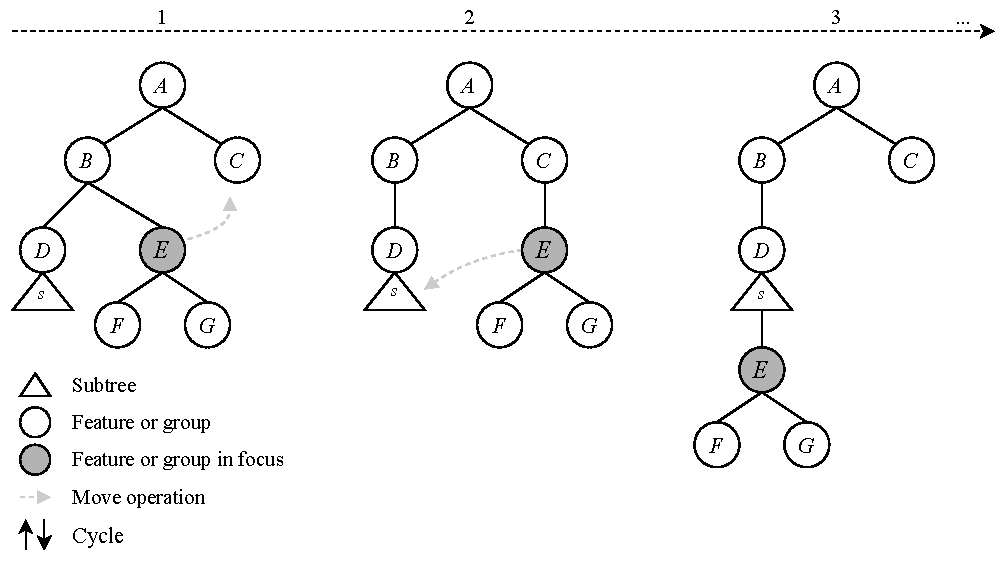
\includegraphics[width=0.9\textwidth]{MoveParadox1}
  \bigskip

  apply \textbf{moveFeature}($D$, $F$) at 1
  \bigskip 
  
  \textbf{Modified plan}
  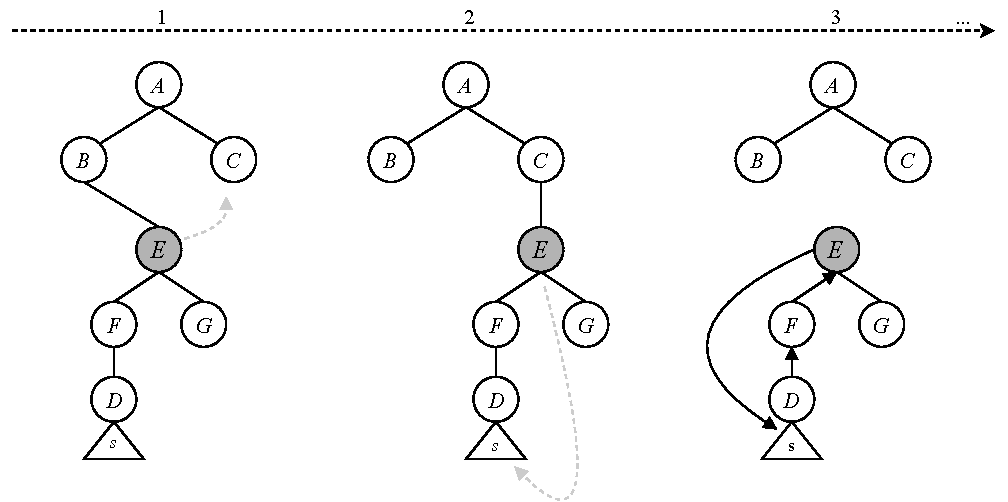
\includegraphics[width=0.9\textwidth]{MoveParadox2}
  \caption{Illustration of move paradox}
  \label{ex:illustration-move-algo}
\end{figure}


First, check whether $n \in \texttt{ancestors}(IBFM, c_1, t_1)$. If this is the case, report that the move causes a cycle and terminate. 

Next, find a list of critical nodes. 
Let $A_n = \texttt{ancestors}(IBFM, n, t_1) = [a_1, a_2, \dots, SN, \dots, r]$ and $A_{c_1} = \texttt{ancestors}(IBFM, c_1, t_1) = [c_2, c_3, \dots, c_n, SN, \dots, r]$ with $SN$ the first common ancestor of $n$ and $c_1$. The list of critical nodes is then $C = [c_1, c_2, \dots, c_n]$, which is essentially the list of $n$'s new ancestors after the move. 

\textbf{Repeat this step until the algorithm terminates:}

Look for the first move of one of the critical nodes. If no such moves occur until $t_e$, the operation causes no paradoxes, and the algorithm terminates successfully.  
  Suppose there is a `move` operation scheduled for $t_k$, with $t_1 < t_k < t_e$, where $c_i$ is moved to $k$. There are two possibilities:  
  \begin{enumerate}
    \item $k$ is in $n$'s subtree, which is equivalent to $n \in \texttt{ancestors}(IBFM, k, t_k)$. Report that the move caused a cycle and terminate. 
\item $k$ is not in $n$'s subtree, so this move is safe. Let $A_k = \texttt{ancestors}(IBFM, k, t_k) = [k_1, k_2, \dots, k_n, SN', \dots, r]$, with SN' the first common element of $A_k$ and $A_n$. Update the list of critical nodes to $[c_1, \dots, c_i, k_1, \dots, k_n]$.
  \end{enumerate}

\begin{figure}[h]
  \begin{minted}[escapeinside=||]{text}
ancestors|$\left((\names{}, \features{}, \groups{}), \, \var{featureID}, t_n \right)$| 
  = let |$\feature \assign     \lookup{\features{}}{\var{featureID}}$|
        parentGroup |$ \assign \lookup{F_p}{t_n} $|
     in 
      case parentGroup of
        { parentGroupID } |$ \rightarrow $| 
          parentGroupID : ancestors|$\left((\names, \features{}, \groups{}), \, \var{parentGroupID}, t_n\right)$|
        |$ \emptyset \rightarrow $| []
ancestors|$\left((\names{}, \features{}, \groups{}), \, \var{groupID}, t_n \right)$| 
  = let |$\group \assign     \lookup{\groups{}}{\var{groupID}}$|
        { parentFeatureID } |$ \assign \lookup{G_p}{t_n} $|
     in 
        parentFeatureID : ancestors|$\left((\names{}, \features{}, groups{}), \, \var{parentFeatureID}, t_n \right)$| 
  \end{minted}
  \caption{\var{ancestors}}
  \label{fun:ancestors}
\end{figure}

The rule identifies the scope $\interval{t_n}{t_{p_2}}$ by looking up the interval in $F_p$ containing $t_n$, and looks up the ID of the original parent group $\lookup{F_p}{\interval{t_n}{t_{p_2}}} = \set{\var{oldParentID}}$. The complex formula checks that the types of the feature and its new parent group are compatible at all times during the temporal scope.

In the conclusion of the rule, the feature's parent map is updated to express that the feature has a new parent during the temporal scope, and the parent groups' subfeature maps are updated similarly.

\section{Move Group Rule}
\label{sec:move-group-rule}
See Figure~\vref{rule:move-group} for the semantics of the \textbf{moveGroup} operation. The semantics is similar to the one for the \textbf{moveFeature} operation, but it differs in that it does not have a check for types. This is because there can only be a conflict between a parent group and a child feature, not a parent feature and a child group. Since only the latter relation changes in this rule, it is not necessary to check that the types are compatible.

\begin{figure}[h]
    \renewcommand{\arraystretch}{1.1}
    \sossize$$\begin{array}{c}
      \ntyperule{Move-Group}
      {\\
        \neg \var{createsCycle} \qquad
        \containing{G_p}{t_n} = \set{\interval{t_{p_1}}{t_{p_2}}} \qquad
        \lookup{G_p}{\interval{t_n}{t_{p_2}}} = \set{\var{oldParentID}} \\
        \lookup{\groups{}}{\var{groupID}} = \group \\
        \lookup{\features{}}{\var{newParentID}} = \feature 
      }
      {
        \textbf{moveGroup}\left( \var{groupID, newParentID}\right) \text{ at } t_n \shove \\
        (\names{}, \features{}, \groups{}) \\
        \transition \\
        \big(\names,\\
        \lookup{\big(\lookup{\features{}}{\var{oldParentID}} \\
        \assign \var{removeGroupAt}(\lookup{\features{}}{\var{oldParentID}}, \interval{t_n}{t_{p_2}}, \var{groupID})\big)}{\var{newParentID}} \\
        \assign 
      \var{addChildGroup}\left(\lookup{\features{}}{\var{newParentID}}, \var{groupID}, t_n\right), \\
        \lookup{\groups{}}{\var{groupID}} \assign \left( G_e,\, G_n,\, G_t,\, 
        \lookup{\var{clampInterval}(G_p, t_n)}{\interval{t_n}{t_{p_2}}} \assign \var{newParentID},\, G_c \right)}
    \end{array}$$
    \caption{The \rulefont{Move-Group} SOS rule}
  \label{rule:move-group}
\end{figure}

\section{Change Feature Variation Type Rule}
\label{sec:change-feature-variation-type-rule}
The rule in Figure~\vref{rule:change-feature-varation-type} shows the semantics of changing the feature variation type of the feature with ID $\var{featureID}$ at time $t_n$. The first expression above the line ($\containing{F_t}{t_n} = \set{\interval{t_{t_1}}{t_{t_2}}}$) identifies the upper bound of the temporal scope, $t_{t_2}$. This is when the feature type was originally planned to change. The next line may be hard to read, but its intent is easier to understand. It checks that all the types a parent group has \emph{while it is the parent of the feature} has a type which is compatible with the new type of the feature. If everything above the line is true, then the $\features{}$ map is updated at $\var{featureID}$ by shortening the interval key for the original type at $t_n$, and assigning the new type to the affected interval $\interval{t_n}{t_{t_2}}$. 

\todo{make it more readable}

\begin{figure}[h]
    \renewcommand{\arraystretch}{1.1}
    \sossize$$\begin{array}{c}
      \ntyperule{Change-Feature-Variation-Type}
      {\\
        \var{featureID} \neq \var{rootID} \qquad
        \containing{F_t}{t_n} = \set{\interval{t_{t_1}}{t_{t_2}}} % Temporal scope = [t_n, t_t_2)
        \\
        \\
        \begin{aligned}
          \forall \interval{t_{p_1}}{t_{p_2}} & \in \overlapping{F_p}{t_n}{t_{t_2}}  \\ % for all parent intervals overlapping the temporal scope
          \forall p & \in \lookup{F_p}{\interval{t_{p_1}}{t_{p_2}}}  \\% for all parent groups (always exactly one) in the parent interval
          \forall t & \in \, \var{getTypes}\left(\lookup{\groups}{p}, \clamp{\interval{t_{p_1}}{t_{p_2}}}{t_n}{t_{t_2}}\right)  \\
                    & \big(\var{compatibleTypes}(t, \var{type})\big) 
        \end{aligned}\\
        \\
        \lookup{\features{}}{\var{featureID}} = \feature
      }
      {
        \textbf{changeFeatureVariationType}\left( \var{featureID}, \var{type}\right) \text{ at } t_n \shove \\
        (\names{}, \features{}, \groups{}) \\
        \transition \\
        (\names{}, \\
        \lookup{\features{}}{\var{featureID}} \assign \left( F_e,\, F_n,\, 
        \lookup{\var{clampInterval}(F_t, t_n)}{\interval{t_n}{t_{t_2}}} \assign \var{type},\, F_p,\, F_c \right),
        \\ \groups{})
      }
    \end{array}$$
    \caption{The \rulefont{Change-Feature-Variation-Type} SOS rule}
    \label{rule:change-feature-varation-type}
\end{figure}

\begin{figure}
  \begin{minted}[escapeinside=||]{text}
getTypes|$\left(\group, \, \interval{t_n}{t_m} \right) = \lookup{G_t}{\interval{t_n}{t_m}}$|
getTypes|$\left(\feature, \, \interval{t_n}{t_m} \right) = \lookup{G_t}{\interval{t_n}{t_m}}$|
  \end{minted}
  \caption{\var{getTypes}}
  \label{get-types}
\end{figure}

\section{Change Group Variation Type Rule}
\label{sec:change-group-variation-type-rule}
The rule in Figure~\vref{rule:change-group-varation-type} is similar to the \textbf{changeFeatureVariationType} rule in Figure~\vref{rule:change-feature-varation-type}, and shows the semantics of changing the type of a group. In a similar way to the aforementioned \textbf{changeFeatureVariationType} rule, it verifies that the types of all the child groups during the affected interval are compatible with the new group type.

\begin{figure}[h]
    \renewcommand{\arraystretch}{1.1}
    \sossize$$\begin{array}{c}
      \ntyperule{Change-Group-Variation-Type}
      {\\
        \containing{G_t}{t_n} = \set{\interval{t_{t_1}}{t_{t_2}}} % Temporal scope = [t_n, t_t_2)
        \\
        \\
        \begin{aligned}
          \forall \interval{t_{c_1}}{t_{c_2}} & \in \overlapping{G_c}{t_n}{t_{t_2}}\\ % for all parent intervals overlapping the temporal scope 
          \forall c & \in \, \bigcup \lookup{G_c}{\interval{t_{c_1}}{t_{c_2}}}\\ % for all child features in the child interval
          \forall t & \in \, \var{getTypes}\left(\lookup{\features}{c}, \clamp{\interval{t_{c_1}}{t_{c_2}}}{t_n}{t_{t_2}}\right) \\ % for all the types of the child features during the temporal scope
                    & \big(\var{compatibleTypes}(\var{type}, t)\big)
      \end{aligned}\\
         \\

        \lookup{\groups{}}{\var{groupID}} = \group
      }
      {
        \textbf{changeGroupVariationType}\left( \var{groupID}, \var{type}\right) \text{ at } t_n \shove \\
        (\names{}, \features{}, \groups{}) \\
        \transition \\
        (\names{}, \features{}, \\
        \lookup{\groups{}}{\var{groupID}} \assign \left( G_e,\, \lookup{\var{clampInterval}(G_t, t_n)}{\interval{t_n}{t_{t_2}}} \assign \var{type},\, G_p,\, G_c \right))
      }
    \end{array}$$
    \caption{The \rulefont{Change-Group-Variation-Type} SOS rule}
  \label{rule:change-group-varation-type}
\end{figure}

\section{Change Feature Name}
\label{sec:change-feature-name}

The semantics of changing the name of a feature are shown in the \rulefont{Change-Feature-Name} rule in Figure~\vref{rule:change-feature-name}. The old name and the next planned name change are identified on the first line ($\lookup{F_n}{t_n} = \set{\var{oldName}}$ and $\containing{F_n}{t_n} = \set{\interval{t_{n_1}}{t_{n_2}}}$ respectively). Since the name must not be in use during the temporal scope, we verify that looking up the new name in the $\names{}$ map returns an empty set. The $\names{}$ map is updated by shortening the interval for the old name to end at $t_n$, and assigning the feature ID to the new name during the temporal scope. Furthermore, the $\features{}$ map is updated at the feature ID, shortening the interval for the old name and assigning the new name to the temporal scope. 

\begin{figure}[h]
    \renewcommand{\arraystretch}{1.1}
    \sossize$$\begin{array}{c}
      \ntyperule{Change-Feature-Name}
      {\\
        \lookup{F_n}{t_n} = \set{\var{oldName}} \qquad
        \containing{F_n}{t_n} = \set{\interval{t_{n_1}}{t_{n_2}}} \\
        \lookup{\lookup{\names{}}{\var{name}}}{\interval{t_n}{t_{n_2}}} = \emptyset \\
        \lookup{\features{}}{\var{featureID}} = \feature
      }
      {
        \textbf{changeFeatureName}\left( \var{featureID}, \var{name}\right) \text{ at } t_n \shove \\
        (\names{}, \features{}, \groups{}) \\
        \transition \\
        \Big(\lookup{\lookup{\big(\lookup{\names{}}{\var{oldName}} \assign \var{clampInterval}\left(\lookup{\names}{\var{oldName}}, t_n\right) \big)}{\var{name}}}{\interval{t_n}{t_{n_2}}} \assign \var{featureID}, \\
        \lookup{\features{}}{\var{featureID}} \assign \left( F_e,\, \lookup{\var{clampInterval}(F_n, t_n)}{\interval{t_n}{t_{n_2}}} \assign \var{name},\, F_t,\, F_p,\, F_c \right), \\
        \groups{}\Big)
      }
    \end{array}$$
    \caption{The \rulefont{Change-Feature-Name} SOS rule}
  \label{rule:change-feature-name}
\end{figure}
